% Options for packages loaded elsewhere
\PassOptionsToPackage{unicode}{hyperref}
\PassOptionsToPackage{hyphens}{url}
%
\documentclass[
]{article}
\usepackage{amsmath,amssymb}
\usepackage{lmodern}
\usepackage{iftex}
\ifPDFTeX
  \usepackage[T1]{fontenc}
  \usepackage[utf8]{inputenc}
  \usepackage{textcomp} % provide euro and other symbols
\else % if luatex or xetex
  \usepackage{unicode-math}
  \defaultfontfeatures{Scale=MatchLowercase}
  \defaultfontfeatures[\rmfamily]{Ligatures=TeX,Scale=1}
\fi
% Use upquote if available, for straight quotes in verbatim environments
\IfFileExists{upquote.sty}{\usepackage{upquote}}{}
\IfFileExists{microtype.sty}{% use microtype if available
  \usepackage[]{microtype}
  \UseMicrotypeSet[protrusion]{basicmath} % disable protrusion for tt fonts
}{}
\makeatletter
\@ifundefined{KOMAClassName}{% if non-KOMA class
  \IfFileExists{parskip.sty}{%
    \usepackage{parskip}
  }{% else
    \setlength{\parindent}{0pt}
    \setlength{\parskip}{6pt plus 2pt minus 1pt}}
}{% if KOMA class
  \KOMAoptions{parskip=half}}
\makeatother
\usepackage{xcolor}
\usepackage[margin=1in]{geometry}
\usepackage{graphicx}
\makeatletter
\def\maxwidth{\ifdim\Gin@nat@width>\linewidth\linewidth\else\Gin@nat@width\fi}
\def\maxheight{\ifdim\Gin@nat@height>\textheight\textheight\else\Gin@nat@height\fi}
\makeatother
% Scale images if necessary, so that they will not overflow the page
% margins by default, and it is still possible to overwrite the defaults
% using explicit options in \includegraphics[width, height, ...]{}
\setkeys{Gin}{width=\maxwidth,height=\maxheight,keepaspectratio}
% Set default figure placement to htbp
\makeatletter
\def\fps@figure{htbp}
\makeatother
\setlength{\emergencystretch}{3em} % prevent overfull lines
\providecommand{\tightlist}{%
  \setlength{\itemsep}{0pt}\setlength{\parskip}{0pt}}
\setcounter{secnumdepth}{-\maxdimen} % remove section numbering
\usepackage{amsmath}
\usepackage{booktabs}
\usepackage{caption}
\usepackage{longtable}
\ifLuaTeX
  \usepackage{selnolig}  % disable illegal ligatures
\fi
\IfFileExists{bookmark.sty}{\usepackage{bookmark}}{\usepackage{hyperref}}
\IfFileExists{xurl.sty}{\usepackage{xurl}}{} % add URL line breaks if available
\urlstyle{same} % disable monospaced font for URLs
\hypersetup{
  pdftitle={American Samoa Model Checks},
  pdfauthor={Meg Oshima},
  hidelinks,
  pdfcreator={LaTeX via pandoc}}

\title{American Samoa Model Checks}
\author{Meg Oshima}
\date{2022-08-22}

\begin{document}
\maketitle

\textbf{This is a summary report for the APRU base model run.}

\hypertarget{model-output}{%
\section{Model Output}\label{model-output}}

\hypertarget{input-data}{%
\subsection{Input Data}\label{input-data}}

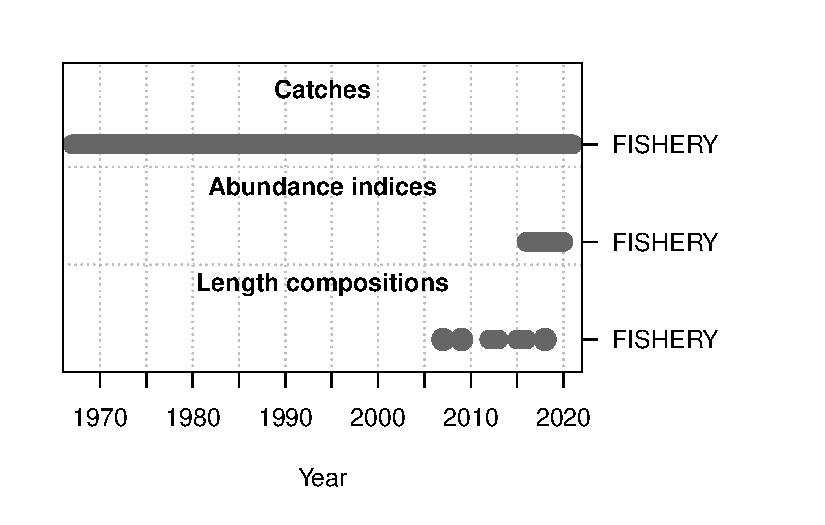
\includegraphics{D:/Marc/Google Drive/02_Work docs/01_Projects/003_AmSam BMUS assessment/AmSam-Bottomfish-2023/SS3 models/APRU/14_F3_NoAdj/0_APRU_14_F3_NoAdj_SS3_Diags_Report_files/figure-latex/unnamed-chunk-2-1.pdf}
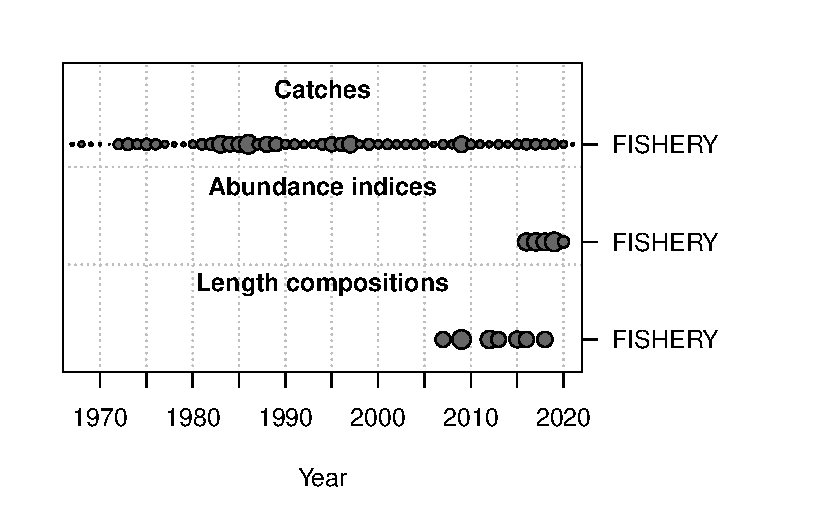
\includegraphics{D:/Marc/Google Drive/02_Work docs/01_Projects/003_AmSam BMUS assessment/AmSam-Bottomfish-2023/SS3 models/APRU/14_F3_NoAdj/0_APRU_14_F3_NoAdj_SS3_Diags_Report_files/figure-latex/unnamed-chunk-2-2.pdf}

\hypertarget{convergence-check}{%
\subsection{Convergence Check}\label{convergence-check}}

\begin{verbatim}
##   Converged      MaxGrad
## 1      TRUE 0.0000552481
\end{verbatim}

\begin{verbatim}
## [1] "1 NOTE:  Max data length bin: 90  < max pop len bins: 100; so will accumulate larger pop len bins"
## [2] "N warnings: 1"
\end{verbatim}

\hypertarget{fit-to-model}{%
\subsection{Fit to Model}\label{fit-to-model}}

\hypertarget{cpue}{%
\subsubsection{CPUE}\label{cpue}}

\begin{center}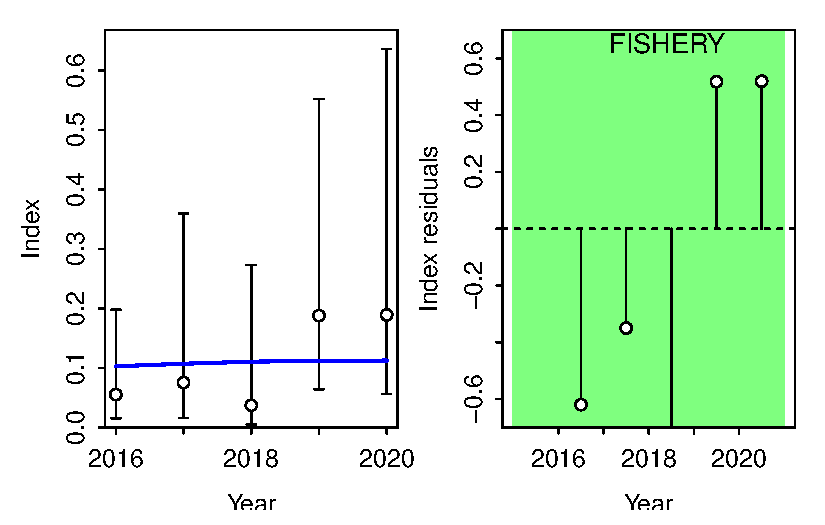
\includegraphics[width=.49\linewidth]{D:\Marc\Google Drive\02_Work docs\01_Projects\003_AmSam BMUS assessment\AmSam-Bottomfish-2023\SS3 models\APRU\14_F3_NoAdj\0_APRU_14_F3_NoAdj_SS3_Diags_Report_files/figure-latex/unnamed-chunk-4-1} \end{center}

\begin{verbatim}
## Residual Runs Test (/w plot) stats by Index:
\end{verbatim}

\begin{verbatim}
## Warning in simpleLoess(y, x, w, span, degree = degree, parametric = parametric, : Chernobyl! trL>n 6

## Warning in simpleLoess(y, x, w, span, degree = degree, parametric = parametric, : Chernobyl! trL>n 6
\end{verbatim}

\begin{verbatim}
## Warning in sqrt(sum.squares/one.delta): NaNs produced
\end{verbatim}

\begin{center}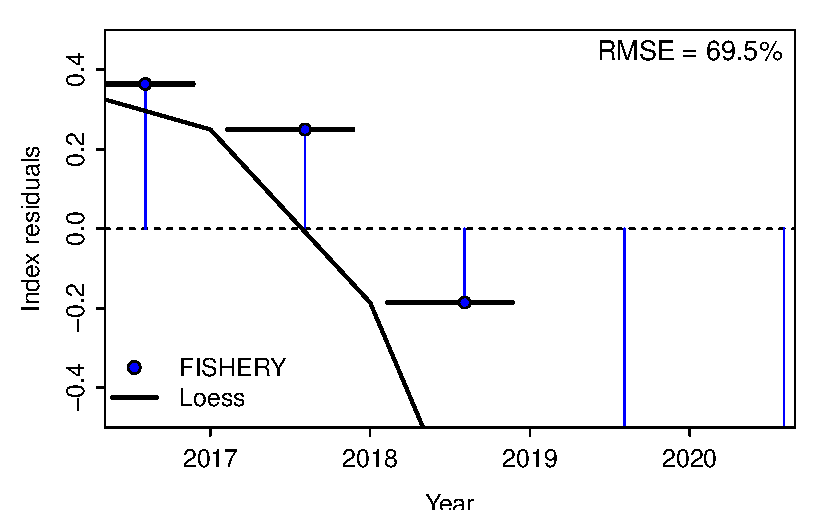
\includegraphics[width=.49\linewidth]{D:\Marc\Google Drive\02_Work docs\01_Projects\003_AmSam BMUS assessment\AmSam-Bottomfish-2023\SS3 models\APRU\14_F3_NoAdj\0_APRU_14_F3_NoAdj_SS3_Diags_Report_files/figure-latex/unnamed-chunk-4-2} \end{center}

\begin{verbatim}
## RMSE stats by Index:
\end{verbatim}

\hypertarget{length-comp}{%
\subsubsection{Length Comp}\label{length-comp}}

\captionsetup[table]{labelformat=empty,skip=1pt}
\begin{longtable}{rrrll}
\toprule
\#Factor & Fleet & New\_Var\_adj & Type & Name \\ 
\midrule
4 & 1 & 0.351585 & len & FISHERY \\ 
\bottomrule
\end{longtable}

\begin{verbatim}
## Residual Runs Test (/w plot) stats by Mean length:
\end{verbatim}

\begin{verbatim}
##     Index runs.p   test  sigma3.lo sigma3.hi type
## 1 FISHERY  0.767 Passed -0.1407916 0.1407916  len
\end{verbatim}

\begin{center}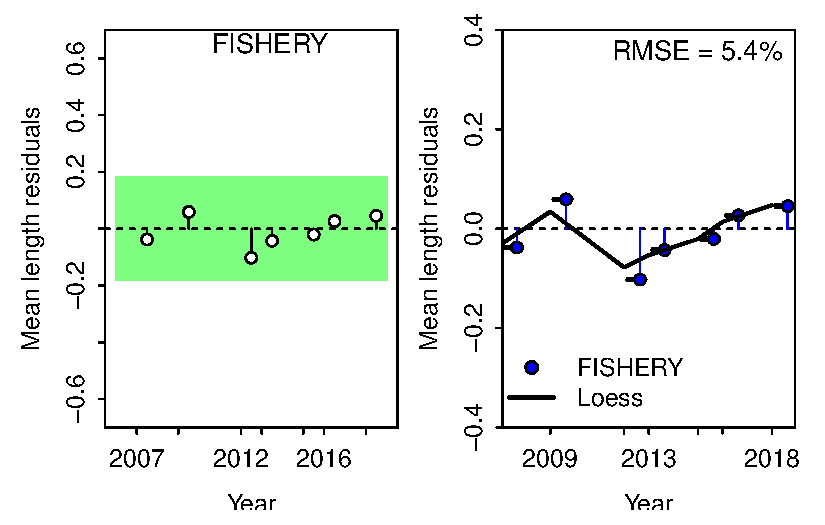
\includegraphics[width=.49\linewidth]{D:\Marc\Google Drive\02_Work docs\01_Projects\003_AmSam BMUS assessment\AmSam-Bottomfish-2023\SS3 models\APRU\14_F3_NoAdj\0_APRU_14_F3_NoAdj_SS3_Diags_Report_files/figure-latex/unnamed-chunk-5-1} \end{center}

\begin{verbatim}
## RMSE stats by Index:
\end{verbatim}

\begin{verbatim}
## # A tibble: 2 x 3
##   Fleet    RMSE.perc  Nobs
##   <chr>        <dbl> <int>
## 1 FISHERY        4.3    12
## 2 Combined       4.3    12
\end{verbatim}

\begin{center}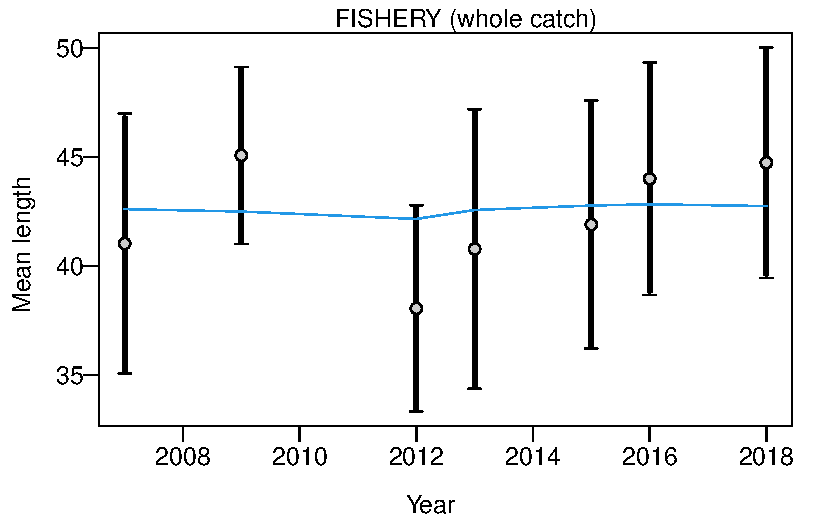
\includegraphics{D:\Marc\Google Drive\02_Work docs\01_Projects\003_AmSam BMUS assessment\AmSam-Bottomfish-2023\SS3 models\APRU\14_F3_NoAdj\0_APRU_14_F3_NoAdj_SS3_Diags_Report_files/figure-latex/unnamed-chunk-6-1} \end{center}

\begin{center}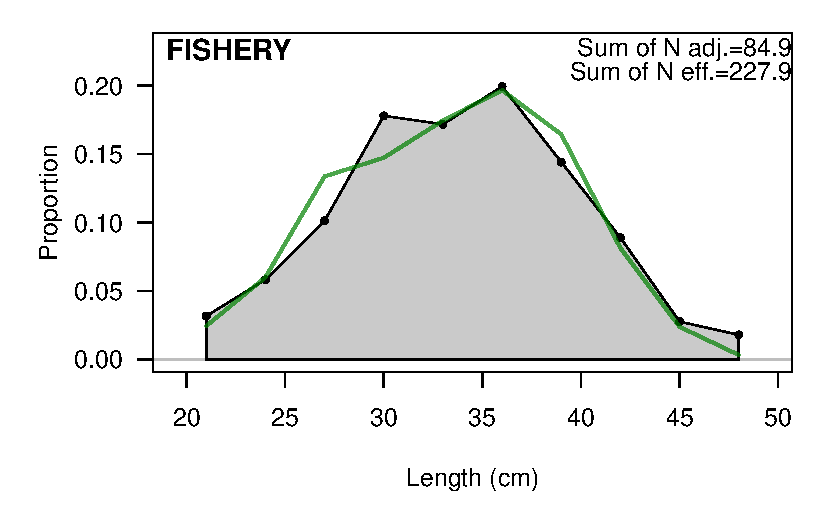
\includegraphics{D:\Marc\Google Drive\02_Work docs\01_Projects\003_AmSam BMUS assessment\AmSam-Bottomfish-2023\SS3 models\APRU\14_F3_NoAdj\0_APRU_14_F3_NoAdj_SS3_Diags_Report_files/figure-latex/unnamed-chunk-6-2} \end{center}

\begin{center}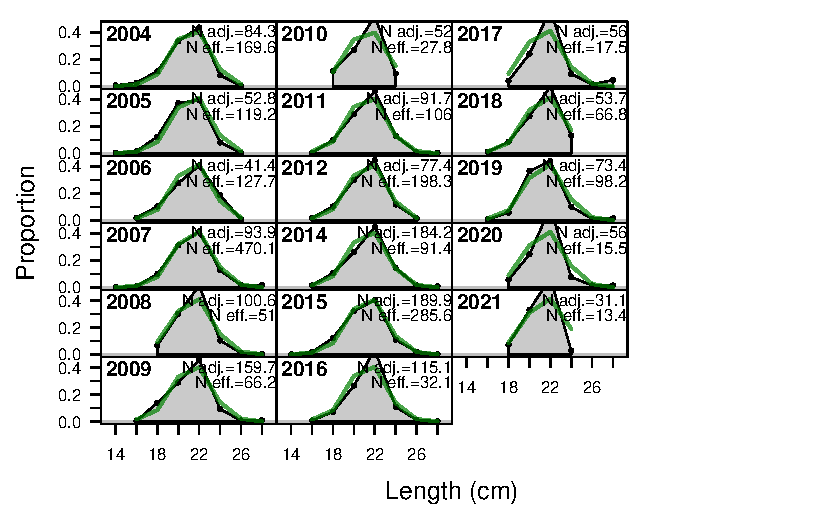
\includegraphics{D:\Marc\Google Drive\02_Work docs\01_Projects\003_AmSam BMUS assessment\AmSam-Bottomfish-2023\SS3 models\APRU\14_F3_NoAdj\0_APRU_14_F3_NoAdj_SS3_Diags_Report_files/figure-latex/unnamed-chunk-6-3} \end{center}

\hypertarget{retrospective-and-hindcasting}{%
\subsection{Retrospective and
Hindcasting}\label{retrospective-and-hindcasting}}

\hypertarget{retrospective}{%
\subsubsection{Retrospective}\label{retrospective}}

\begin{verbatim}
## Error in xy.coords(x, y, setLab = FALSE): 'x' and 'y' lengths differ
\end{verbatim}

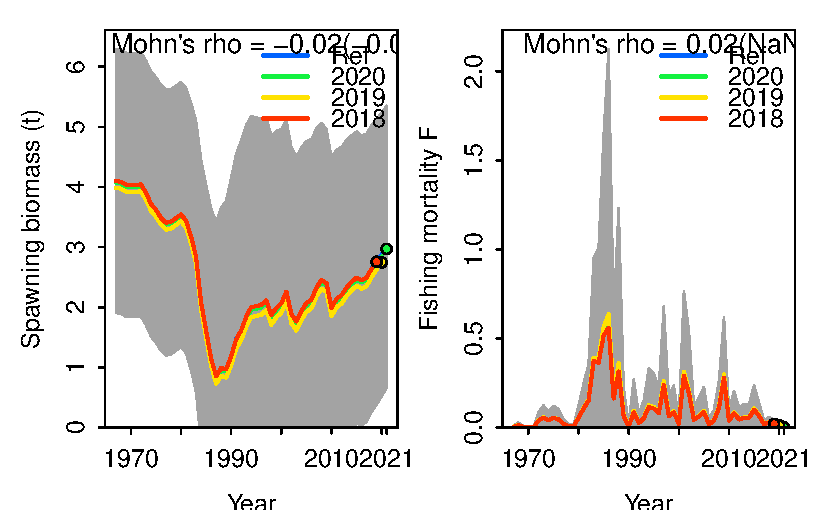
\includegraphics{D:/Marc/Google Drive/02_Work docs/01_Projects/003_AmSam BMUS assessment/AmSam-Bottomfish-2023/SS3 models/APRU/14_F3_NoAdj/0_APRU_14_F3_NoAdj_SS3_Diags_Report_files/figure-latex/unnamed-chunk-7-1.pdf}

\hypertarget{hindcasting}{%
\subsubsection{Hindcasting}\label{hindcasting}}

\begin{verbatim}
## Plotting Hindcast Cross-Validation (one-step-ahead) 
## 
##  Computing MASE with only 2 of 3  prediction residuals for Index FISHERY 
## 
##  Warning:  Unequal spacing of naive predictions residuals may influence the interpretation of MASE
\end{verbatim}

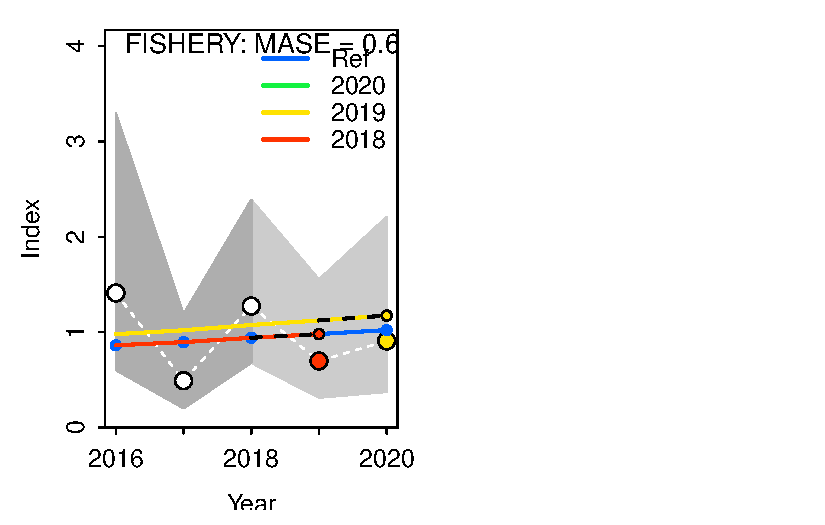
\includegraphics{D:/Marc/Google Drive/02_Work docs/01_Projects/003_AmSam BMUS assessment/AmSam-Bottomfish-2023/SS3 models/APRU/14_F3_NoAdj/0_APRU_14_F3_NoAdj_SS3_Diags_Report_files/figure-latex/unnamed-chunk-8-1.pdf}

\begin{verbatim}
## 
## MASE stats by Index:
## Plotting Hindcast Cross-Validation (one-step-ahead) 
## 
## No observations in evaluation years to compute prediction residuals for Index FISHERY 
## 
## MASE stats by Index:
\end{verbatim}

\hypertarget{recruitment-deviations}{%
\subsection{Recruitment Deviations}\label{recruitment-deviations}}

\begin{verbatim}
## Skipped SSplotrecdevs - no rec devs estimated
\end{verbatim}

\hypertarget{likelihood-profile}{%
\subsection{Likelihood Profile}\label{likelihood-profile}}

\begin{verbatim}
## [1] "SR_LN"
\end{verbatim}

\begin{verbatim}
## Parameter matching profile.string=SR_LN: SR_LN(R0)
\end{verbatim}

\begin{verbatim}
## Parameter values (after subsetting based on input 'models'): 0.2, 0.3, 0.4, 0.5, 0.6, 0.7, 0.8, 0.9, 1, 1.1, 1.2, 1.3, 1.4, 1.5, 1.6, 1.05777
\end{verbatim}

\begin{verbatim}
## 
## Likelihood components showing max change as fraction of total change.
## To change which components are included, change input 'minfraction'.
\end{verbatim}

\begin{verbatim}
##                      frac_change include                            label
## TOTAL                     1.0000    TRUE                            Total
## Catch                     0.0000   FALSE                            Catch
## Equil_catch               0.0000   FALSE                Equilibrium catch
## Survey                    0.0100    TRUE                       Index data
## Length_comp               0.9899    TRUE                      Length data
## Recruitment               0.0000   FALSE                      Recruitment
## InitEQ_Regime             0.0000   FALSE Initital equilibrium recruitment
## Forecast_Recruitment      0.0000   FALSE             Forecast recruitment
## Parm_priors               0.0000   FALSE                           Priors
## Parm_softbounds           0.0001   FALSE                      Soft bounds
## Parm_devs                 0.0000   FALSE             Parameter deviations
## Crash_Pen                 0.0000   FALSE                    Crash penalty
\end{verbatim}

\begin{verbatim}
## Parameter matching profile.string = 'SR_LN': 'SR_LN(R0)
## Parameter values (after subsetting based on input 'models'): 0.2, 0.3, 0.4, 0.5, 0.6, 0.7, 0.8, 0.9, 1, 1.1, 1.2, 1.3, 1.4, 1.5, 1.6, 1.05777,
\end{verbatim}

\begin{verbatim}
## Fleet-specific likelihoods showing max change as fraction of total change.
## To change which components are included, change input 'minfraction'.
##                       frac_change include
## prof.table....c.1.3..           1    TRUE
\end{verbatim}

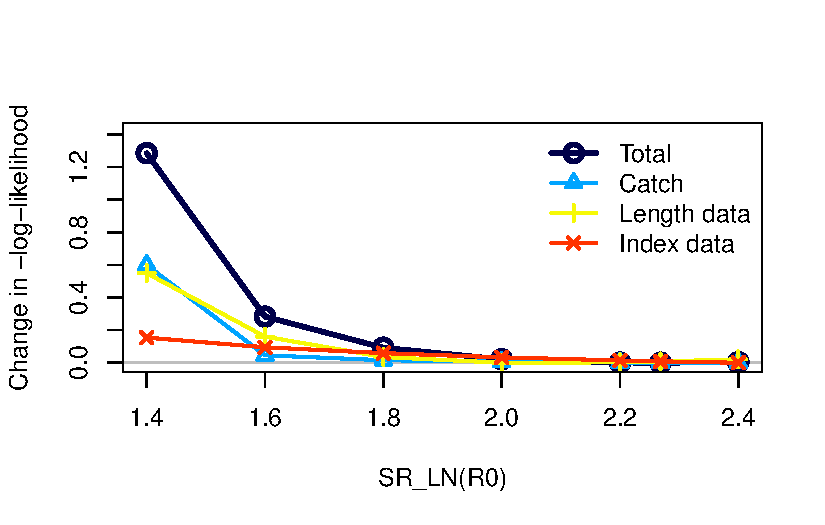
\includegraphics{D:/Marc/Google Drive/02_Work docs/01_Projects/003_AmSam BMUS assessment/AmSam-Bottomfish-2023/SS3 models/APRU/14_F3_NoAdj/0_APRU_14_F3_NoAdj_SS3_Diags_Report_files/figure-latex/unnamed-chunk-10-1.pdf}
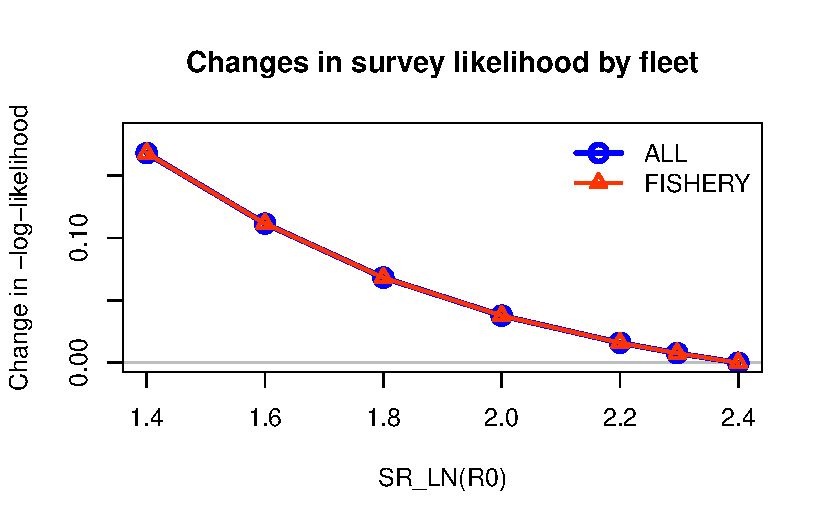
\includegraphics{D:/Marc/Google Drive/02_Work docs/01_Projects/003_AmSam BMUS assessment/AmSam-Bottomfish-2023/SS3 models/APRU/14_F3_NoAdj/0_APRU_14_F3_NoAdj_SS3_Diags_Report_files/figure-latex/unnamed-chunk-10-2.pdf}

\hypertarget{management-quantities}{%
\subsection{Management Quantities}\label{management-quantities}}

\begin{verbatim}
## 
##  starter.sso with Bratio: SSB/SSBMSY and F: _abs_F 
## 
\end{verbatim}

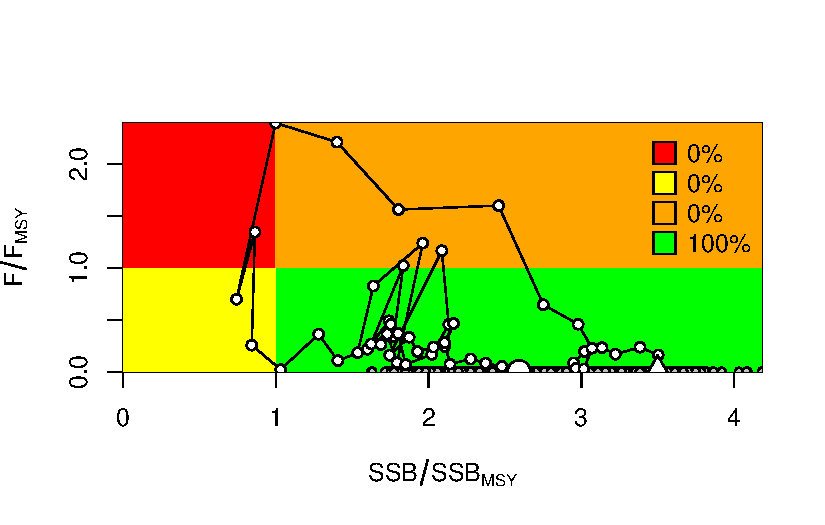
\includegraphics{D:/Marc/Google Drive/02_Work docs/01_Projects/003_AmSam BMUS assessment/AmSam-Bottomfish-2023/SS3 models/APRU/14_F3_NoAdj/0_APRU_14_F3_NoAdj_SS3_Diags_Report_files/figure-latex/unnamed-chunk-11-1.pdf}

\begin{verbatim}
## Plot Comparison of stock
\end{verbatim}

\begin{verbatim}
## Plot Comparison of harvest
\end{verbatim}

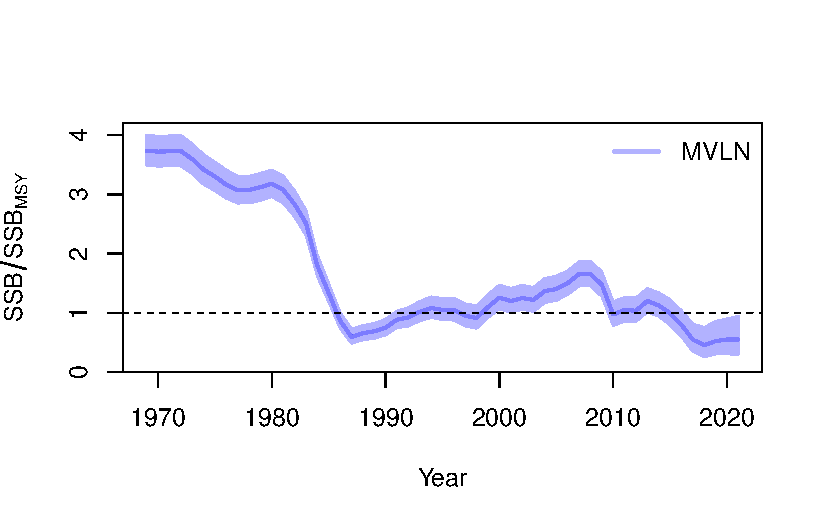
\includegraphics{D:/Marc/Google Drive/02_Work docs/01_Projects/003_AmSam BMUS assessment/AmSam-Bottomfish-2023/SS3 models/APRU/14_F3_NoAdj/0_APRU_14_F3_NoAdj_SS3_Diags_Report_files/figure-latex/unnamed-chunk-11-2.pdf}

\begin{verbatim}
## Plot Comparison of SSB
\end{verbatim}

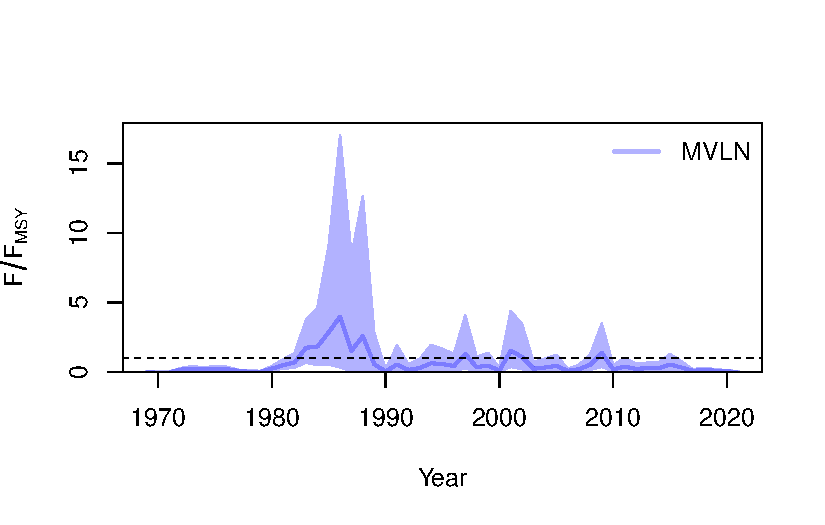
\includegraphics{D:/Marc/Google Drive/02_Work docs/01_Projects/003_AmSam BMUS assessment/AmSam-Bottomfish-2023/SS3 models/APRU/14_F3_NoAdj/0_APRU_14_F3_NoAdj_SS3_Diags_Report_files/figure-latex/unnamed-chunk-11-3.pdf}

\begin{verbatim}
## Plot Comparison of F
\end{verbatim}

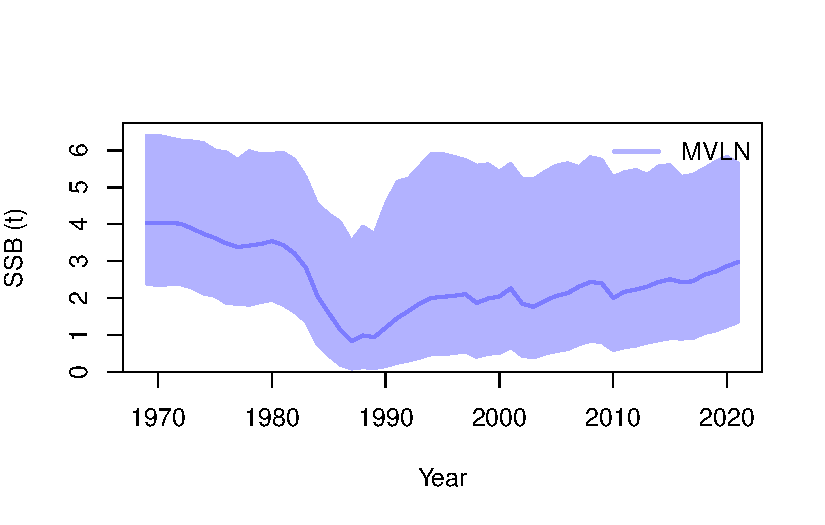
\includegraphics{D:/Marc/Google Drive/02_Work docs/01_Projects/003_AmSam BMUS assessment/AmSam-Bottomfish-2023/SS3 models/APRU/14_F3_NoAdj/0_APRU_14_F3_NoAdj_SS3_Diags_Report_files/figure-latex/unnamed-chunk-11-4.pdf}
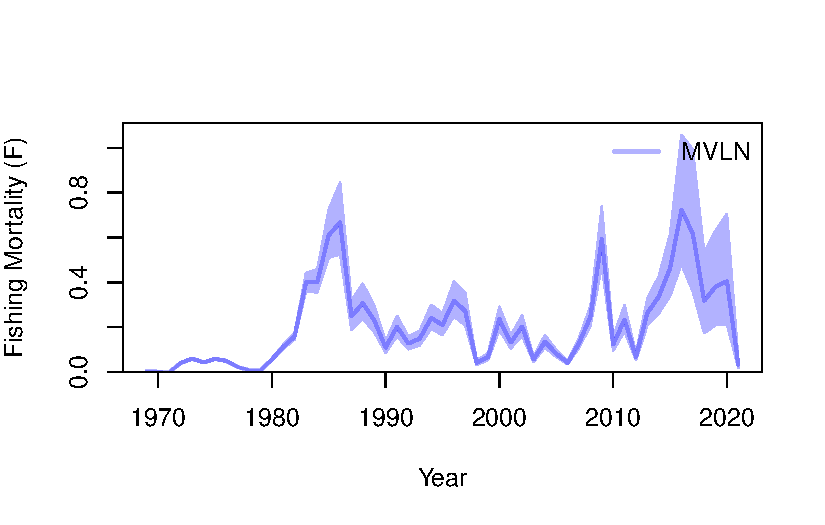
\includegraphics{D:/Marc/Google Drive/02_Work docs/01_Projects/003_AmSam BMUS assessment/AmSam-Bottomfish-2023/SS3 models/APRU/14_F3_NoAdj/0_APRU_14_F3_NoAdj_SS3_Diags_Report_files/figure-latex/unnamed-chunk-11-5.pdf}

\begin{verbatim}
## RStudioGD 
##         2
\end{verbatim}

\hypertarget{jitter}{%
\subsection{Jitter}\label{jitter}}

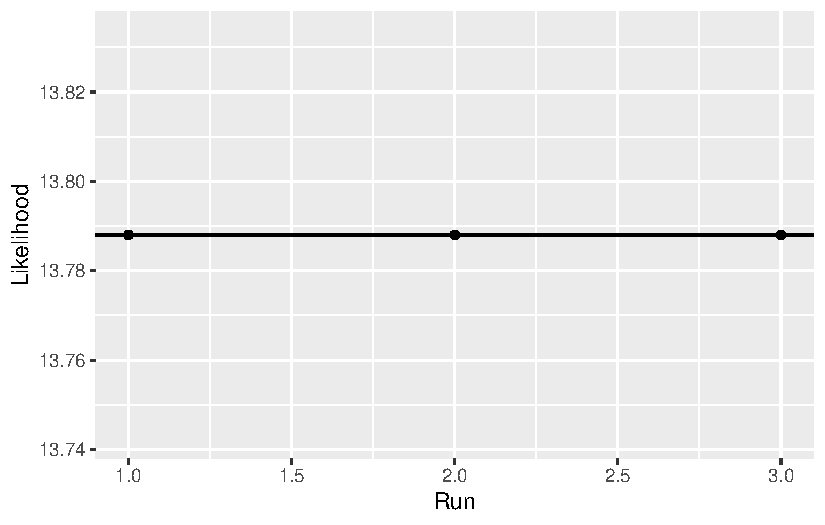
\includegraphics{D:/Marc/Google Drive/02_Work docs/01_Projects/003_AmSam BMUS assessment/AmSam-Bottomfish-2023/SS3 models/APRU/14_F3_NoAdj/0_APRU_14_F3_NoAdj_SS3_Diags_Report_files/figure-latex/unnamed-chunk-12-1.pdf}

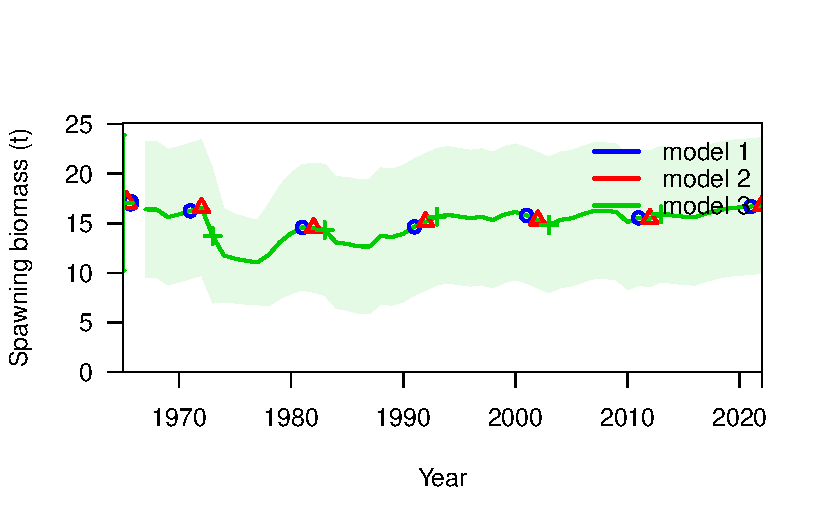
\includegraphics{D:/Marc/Google Drive/02_Work docs/01_Projects/003_AmSam BMUS assessment/AmSam-Bottomfish-2023/SS3 models/APRU/14_F3_NoAdj/0_APRU_14_F3_NoAdj_SS3_Diags_Report_files/figure-latex/unnamed-chunk-13-1.pdf}
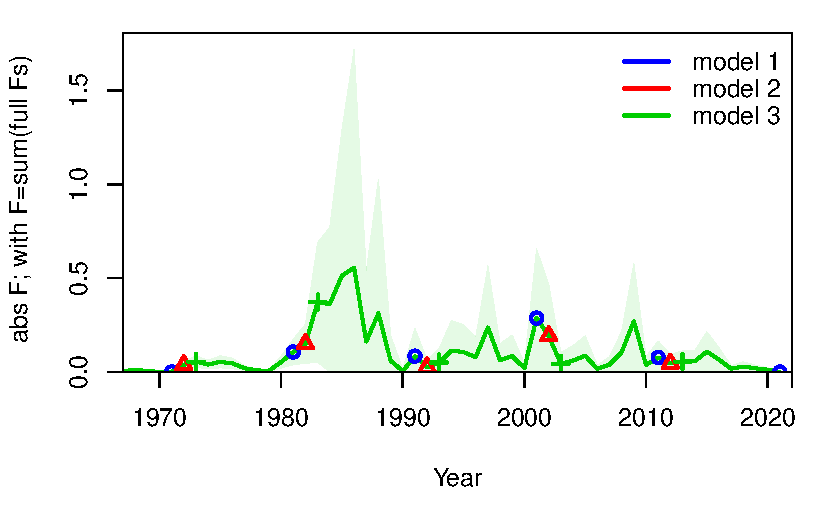
\includegraphics{D:/Marc/Google Drive/02_Work docs/01_Projects/003_AmSam BMUS assessment/AmSam-Bottomfish-2023/SS3 models/APRU/14_F3_NoAdj/0_APRU_14_F3_NoAdj_SS3_Diags_Report_files/figure-latex/unnamed-chunk-13-2.pdf}
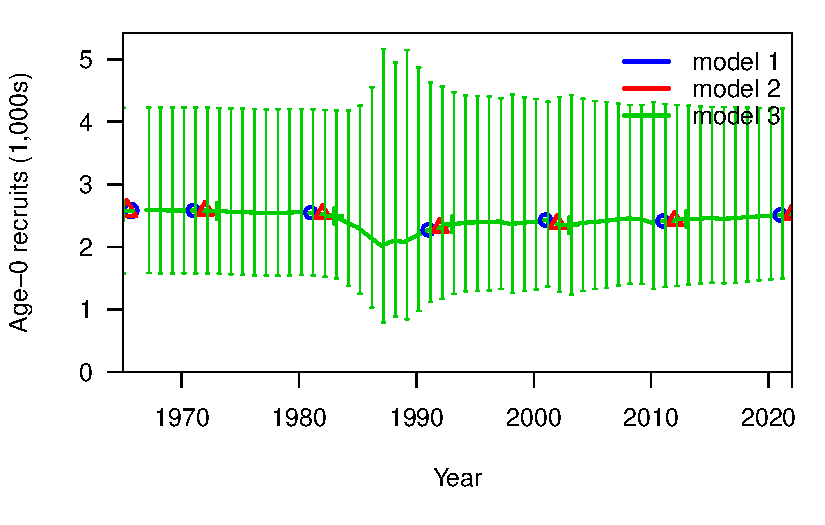
\includegraphics{D:/Marc/Google Drive/02_Work docs/01_Projects/003_AmSam BMUS assessment/AmSam-Bottomfish-2023/SS3 models/APRU/14_F3_NoAdj/0_APRU_14_F3_NoAdj_SS3_Diags_Report_files/figure-latex/unnamed-chunk-13-3.pdf}

\hypertarget{section}{%
\subsection{}\label{section}}

\end{document}
